\chapter{简洁}
赘语是写作的疾患。我们的社会充斥着赘词、循环结构、浮夸的修饰,以及毫无意义的行话。

有谁能明白美国混乱呆板的日常商业用语?比如:备忘录、公司报告、商务信函、解释其最新“简化”账目的银行通知单。哪位保险或医疗计划参保成员能搞清楚手册上所解释的费用与受益情况?哪位父母能按照包装盒上的说明拼装起孩子的玩具?举国上下的趋势都是夸大其词,因而听起来显得重要。航班飞行员通告人们,他目前预感将会经历相当大的降雨,而他决不会说可能要下雨。因为这样句子就太简单了,这么说一定会有不妥之处。

但是好的写作的秘诀就是剥离每一句话中的杂物,只存留其最洁净的部分。每一个无用之词、每一个可短的长词、每一个在动词中已经表示其相同意思的副词、每一个使读者不知谁在干什么的被动语态结构——这些都是削弱句子力度的成千上万种掺杂物。而且这些通常与教育程度和官衔大小成正比。

20世纪60年代,我所在的大学校长在一阵校园骚乱之后为安抚校友写了一封信。他是这样开头的,“你们也许意识到,我们经历了非常大的具有潜在爆炸性的对只是部分相关问题不满而产生的表现方式。”他的意思是学生们在诸多方面与校方纠缠不休。相比于学生们潜在的爆炸性的不满表现,我更不满于校长的英文。以下是美国联邦政府1942年的灯火管制令:

必须做好以下准备,在空袭期间,完全遮挡好所有联邦政府建筑以及联邦政府所用的非联邦政府建筑,防止内外照明暴露。

罗斯福总统设法将其改成了备忘录,他是这样改的:“告诉大家遮挡好昼夜办公建筑的窗户。”我反倒更喜欢富兰克林·罗斯福总统的方式。

简洁,再简洁。梭罗就是这样提醒大家的。没有哪位美国作家像梭罗那样持之以恒地践行其布道。翻开《瓦尔登湖》的任何一页,你都能发现有人用简明质朴、有条有理的方式讲述自己的感悟:

我走入林地,因为我希望能明明白白地活,只面对生活的基本需求,看看是否能学到生活的教诲,而不要到临死时才发现自己并没有活过。

我们其他人又如何避免赘语以取得这种令人羡慕的自由呢?回答是,将赘语清除出头脑。清晰的思考产生清晰的写作。两者缺一不可。思维混沌的人不可能写好。他也许能写好开头一两段,但很快读者就会不知所云,而这简直就是滔天大罪,因为读者可不会那么容易就被吸引回来。

那么这个逃之夭夭的家伙,这位读者又是谁呢?读者的注意力只能持续约三十秒——有众多的力量争夺其注意力。曾几何时,这些力量还相对有限:报纸、杂志、收音机、配偶、孩子、宠物等。而今这些力量还包括星云般众多的获取娱乐和信息的电子设备——电视、VCR、DVD、CD、电子游戏、互联网、电子邮件、手机、黑莓电子产品、苹果随身听——也包括健身计划、游泳池、草地,还有最强有力的竞争对手,犯困。有些人坐在椅子上拿着杂志或书打盹,那是由于作者使其不堪重负。

我们不该说读者太笨或太懒,跟不上思路。假如读者不知所云,一般是因为作者不够细心。作者的粗心大意有多种表现。也许一句话毫无头绪,读者即使砍出一条路来,仍是一头雾水。也许一句话构造拙劣,读者可以有几种理解。也许作者在句中偷换代词、偷换时态,使读者迷失于谁在说话或事情是何时发生的。也许B句不是A句的逻辑衔接部分,作者在头脑中清楚彼此之间的关系,但却没有注意提供有效的连接词。也许作者用词错误,也不屑查词典。

面对这些障碍,读者起初还耐着性子。他们责备自己——显然是自己没读懂,然后重读费解的句子或整段,就像拼凑古代如尼文\footnote{rune,神秘晦涩的古代北欧文字。}一样,边猜边接着读。但这样做的时间不会长。作者叫读者太吃力了,因而读者会找寻技艺更高的作者。

因此作者必须不断地问:我想说什么?令人吃惊的是,一些作者常常不知道自己想说什么。那么他们就必须看看自己写了什么,然后问:我说过这个了吗?首次接触这个题目的读者能明白吗?如果不能,那就是其中有什么模糊不清的东西钻入其运转之中。清晰的作家一定会头脑清醒地看到那东西是什么:模糊。

我并不是说有人天生就头脑清楚、是作家的料,而其他人天生就迷糊,永远写不好。清晰地思考是一种自觉的行为,作者必须练就这一本领,就像他们做任何需要逻辑思维的事情时一样,如列一个购物单,或作代数题。好的写作并不是与生俱来的,但多数人却似乎认为如此。专业作家总是遭人挑衅,那些人会说自己也想“有朝一日写点什么”——意思是等他们从自己真正的职业退休后再点儿什么,比如保险或地产那些难做的职业。或者他们会说,“对此我都能写一本书了。”我表示怀疑。

写作是艰苦的工作。一个表达清晰的句子绝非偶然。很少有句子是第一次甚或第三次写出来就对路。写作绝望时请记住这个。如果你觉得写作难,那是因为它确实难。

\begin{figure}[!htb]
\centering
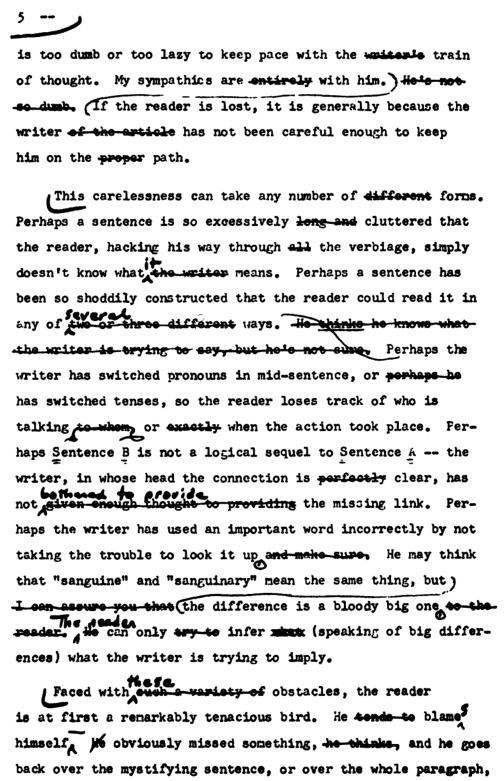
\includegraphics[width=0.9\textwidth]{figure/fig1-1.png}
\end{figure}


\begin{figure}[!htb]
\centering
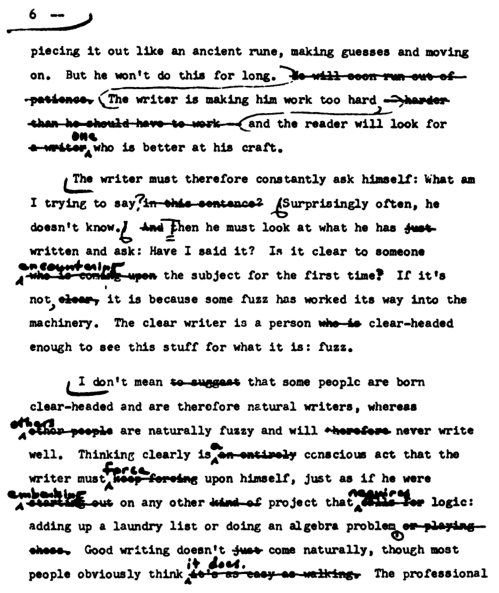
\includegraphics[width=0.9\textwidth]{figure/fig1-2.png}
\end{figure}


以上是《写作法宝》第一版本章终稿的两页。虽然这两页看起来像第一稿,其实已经修改和重新打过四五遍了——几乎每隔一页都是如此。每次修改我都尽力使所写的文字更紧凑、有力、精确,剔除所有无用的部分。然后再过一遍,朗读一遍,每次都惊讶地发现仍有许多赘词可以去除。(在后几版中,我去除了用来表示“作者”与“读者”的性别歧视性代词“他”。)